\chapter{DevOps-Integrated Cloud Architecture Design}
\minitoc
\newpage

\setcounter{secnumdepth}{0} % Set the section counter to 0 so next section is not counted in toc
% ----------------------- Introduction ----------------------- %
\section{Introduction}
This chapter covers the architectural decisions made throughout the project. 
It reviews the most widely used tools and technologies in the industry for 
each component of the solution, and for each one a comparison is made to 
justify the choice adopted. These choices then form the foundation of the 
proposed architecture, which describes how all selected technologies are 
assembled together to address the limitations identified in the previous chapter.

\setcounter{secnumdepth}{2} % Resume counting the sections for the toc with a depth of 2 (Sections and sub-sections)
% ----------------------------------- SECTIONS (v) ----------------------------------- 
% ----------------------- Comparative Analysis ----------------------- %
\section{General Concepts}
To implement a scalable and automated infrastructure, a range of tools is
required for version control, container management, deployment orchestration,
and cloud provisioning. In this section, we provide a comparative study of
widely used tools and cloud platforms in the industry, highlighting their
main characteristics and advantages. This analysis allows us to identify
which solutions are most suitable for modernizing and automating the
deployment of applications in cloud environments.

%The Infrastructure Foundation
\subsection{Cloud Infrastructure}
In this section, we discuss two essential concepts of modern cloud environments. 
The first concerns cloud service providers, while the second focuses on the concept 
of Infrastructure as Code (IaC), which enables the automation of infrastructure 
management and deployment.

\subsubsection*{\underline{Cloud Providers}}
Modern scalable applications rely on cloud platforms to provide on-demand
resources, high availability, and automated infrastructure management. The
three leading providers are Amazon Web Services (AWS) \cite{aws}, Microsoft Azure \cite{azure},
and Google Cloud Platform (GCP) \cite{gcp}. Each offers a wide range of services for
compute, storage, networking, monitoring, and deployment automation, as summarized 
in Table \ref{tab:cloud_providers}.

\begin{table}[H]
    \renewcommand{\arraystretch}{1.5}%
    \caption{Comparative study between AWS, Azure, and GCP}
    \label{tab:cloud_providers}
    \centering
    \medskip
    \begin{tabularx}{\textwidth} {
            | >{\centering\arraybackslash}p{2cm}
            | >{\justifying\arraybackslash}X
            | >{\justifying\arraybackslash}X
            | >{\justifying\arraybackslash}X |}
        \hline
        \rowcolor{primary} \textbf{Aspect} & \textbf{AWS} & \textbf{Azure} & \textbf{GCP} \\
        \hline
        \textbf{Overview} & AWS is the most mature and widely adopted cloud platform, offering a comprehensive ecosystem of services. & Azure integrates tightly with Microsoft products and enterprise environments, making it ideal for companies using Windows-based infrastructures. & GCP is known for strong data analytics, AI/ML services, and competitive pricing for compute and storage. \\
        \hline
        \textbf{Advantages} & \begin{itemize}[leftmargin=*, topsep=0pt, itemsep=1pt, parsep=2pt]
            \item Largest service ecosystem
            \item Mature DevOps and deployment tools
            \item Global reach and reliability
        \end{itemize} & \begin{itemize}[leftmargin=*, topsep=0pt, itemsep=1pt, parsep=2pt]
            \item Strong integration with Microsoft software
            \item Enterprise-friendly security and compliance
            \item Hybrid cloud support
        \end{itemize} & \begin{itemize}[leftmargin=*, topsep=0pt, itemsep=1pt, parsep=2pt]
            \item Advanced data analytics and AI/ML capabilities
            \item Competitive pricing for compute and storage
            \item Fast-growing ecosystem with strong Kubernetes support
        \end{itemize} \\
        \hline
        \textbf{Disadvantages} & Cost can be high for small deployments; complexity can be overwhelming. & Smaller ecosystem than AWS; some services lag behind AWS in features. & Smaller global infrastructure; fewer enterprise integrations than AWS or Azure. \\
        \hline
    \end{tabularx}
\end{table}

All three providers support the core requirements of scalable, automated,
and highly available applications. For our internship project, AWS was chosen
due to the company’s existing usage of its services, team familiarity, and
strong ecosystem for DevOps and cloud-native practices.

\subsubsection*{\underline{Infrastructure as Code}}
Infrastructure as Code (IaC) is the practice of defining and provisioning cloud 
resources through code rather than manual configuration. This approach makes 
infrastructure reproducible, versionable, and easier to automate. Two leading 
IaC tools are discussed: Terraform and AWS CloudFormation. Table \ref{tab:iac_tools} 
illustrates a comparative study of these tools.

\begin{table}[H]
    \renewcommand{\arraystretch}{1.5}%
    \caption{Comparative study between Terraform and CloudFormation}
    \label{tab:iac_tools}
    \centering
    \medskip
    \begin{tabularx}{1\textwidth} {
            | >{\hsize=.7\hsize\linewidth=\hsize\centering\arraybackslash}X
            | >{\hsize=1.15\hsize\linewidth=\hsize\justifying\arraybackslash}X
            | >{\hsize=1.15\hsize\linewidth=\hsize\justifying\arraybackslash}X |}
        \hline
        \rowcolor{primary} \textbf {Aspect} & \textbf{Terraform}                                                                                                                                                                                                                     & \textbf{CloudFormation}                                                                                                                                                                                                                                           \\
        \hline
        \textbf {Overview}                  & \noindent An open-source IaC tool by HashiCorp that uses the declarative HCL language. It supports multiple cloud providers through a plugin-based provider system.                                                                                                             & \noindent AWS's native IaC service that provisions and manages AWS resources using JSON or YAML templates. It is tightly integrated with the AWS ecosystem.                                                                                                                                                                                   \\
        \hline
        \textbf {Advantages}                & \begin{itemize}[leftmargin=*, topsep=0pt, itemsep=1pt, parsep=2pt]
            \item Cloud-agnostic (supports AWS, Azure, GCP, etc.)
            \item Modular structure with reusable modules
            \item Plan command previews changes before applying
            \item Large community and extensive provider ecosystem
        \end{itemize} & \begin{itemize}[leftmargin=*, topsep=0pt, itemsep=1pt, parsep=2pt]
            \item Deep AWS integration with no extra tooling
            \item Automatic rollback on deployment failures
            \item Free to use (pay only for provisioned resources)
            \item Drift detection built in
        \end{itemize}                                                \\
        \hline
        \textbf {Disadvantages}             & \noindent State file management requires careful handling; the HCL language has its own learning curve.                                                                                                                                                                                                        & \noindent Locked to AWS only; verbose template syntax; slower to adopt new AWS features compared to Terraform providers. \\
        \hline
    \end{tabularx}
\end{table}

Terraform was selected for this project due to its position as an industry 
standard for infrastructure as code \cite{terraform_adoption}. Unlike tools 
that are tied to a specific cloud provider, Terraform works with all major 
providers, which avoids vendor lock-in and ensures that the infrastructure 
knowledge built throughout this project remains usable regardless of the 
platform chosen in the future.

%Compute & Orchestration
\subsection{Containerization and Orchestration}
This section covers two fundamental concepts of modern application deployment. 
The first concerns container management, which introduces the technology used 
to package and run applications in isolated environments. The second focuses 
on container orchestration, presenting the main tools used to manage containers 
at scale and concluding with the approach adopted for this project.

\subsubsection*{\underline{Container Management:}}
There are many container management technologies available today. 
The two most widely used are Docker and Podman, each offering a 
different approach to building and running containers.

\begin{table}[H]
    \renewcommand{\arraystretch}{1.5}%
    \caption{Comparative study between Docker and Podman}
    \centering
    \medskip
    \begin{tabularx}{1\textwidth} {
            | >{\hsize=.7\hsize\linewidth=\hsize\centering\arraybackslash}X
            | >{\hsize=1.15\hsize\linewidth=\hsize\justifying\arraybackslash}X
            | >{\hsize=1.15\hsize\linewidth=\hsize\justifying\arraybackslash}X |}
        \hline
        \rowcolor{primary} \textbf {Aspect} & \textbf {Docker}                                                                                                                                                                                                                    & \textbf {Podman}                                                                                                                                                                      \\
        \hline
        \textbf {Definition}                & \multicolumn{2}{|>{\hsize=2.35\hsize}X|} {Docker and Podman are both  container management technologies used to build container images and store said images in a registry to then run them as containers in a target environment.}                                                                                                                                                                                         \\
        \hline
        \textbf {Technology}                & \noindent Docker uses the containerd daemon which does the pulling of images then hands over the creation process to a low-level runtime named runc.                                                                                & \noindent Podman uses a daemon-less approach using a technology named conmon which does the heavy lifting. It also delegates the container creation to a low-level container runtime. \\
        \hline
        \textbf {Specificity}               & \noindent Docker Desktop is a great feature for Docker which provides an easy way to build and distribute containers amongst developers.                                                                                            & \noindent The smallest unit in Podman is the pod. A pod is the organizational unit for containers and is directly compatible with Kubernetes.                                         \\
        \hline
    \end{tabularx}
\end{table}
We can see the similarities between the two technologies and in theory, it shouldn't really matter which one we choose since both Docker and Podman are inter-changeable.

\subsubsection*{\underline{Container Orchestration:}}
Container orchestration is the automated management of containerized applications 
across multiple machines, handling deployment, scaling, networking, and recovery. 
After reviewing the available container orchestration solutions, the choice 
was narrowed down to two main candidates: Docker Swarm and Kubernetes.

\begin{table}[H]
    \renewcommand{\arraystretch}{1.5}%
    \caption{Comparative study between Docker Swarm and Kubernetes}
    \centering
    \medskip
    \begin{tabularx}{1\textwidth} {
            | >{\hsize=.7\hsize\linewidth=\hsize\centering\arraybackslash}X
            | >{\hsize=1.15\hsize\linewidth=\hsize\justifying\arraybackslash}X
            | >{\hsize=1.15\hsize\linewidth=\hsize\justifying\arraybackslash}X |}
        \hline
        \rowcolor{primary} \textbf {Aspect} & \textbf{Docker Swarm}                                                                                                                                                                                                                                                              & \textbf{Kubernetes}                                                      \\
        \hline
        \textbf {Overview}                  & \multicolumn{2}{|>{\hsize=2.35\hsize}X|} {Docker Swarm is a lightweight, easy-to-use orchestration tool with limited offerings compared to Kubernetes. In contrast, Kubernetes is complex but powerful and it provides self-healing and auto-scaling capabilities out of the box \cite{comparative_orchestration_2024}.}                                                                            \\
        \hline
        \textbf {Advantages}                & \begin{itemize}[leftmargin=*, topsep=0pt, itemsep=1pt, parsep=2pt]
            \item Straightforward to install
            \item Takes less time to learn
            \item Works with the Docker CLI
        \end{itemize}                                                                                                                                                                                                                                                          & \begin{itemize}[leftmargin=*, topsep=0pt, itemsep=1pt, parsep=2pt]
            \item Can sustain and manage large architectures and complex workloads
            \item Has a self-healing capacity that supports automatic scaling.
            \item Supports every operating system.
            \item Has a large open-source community with Google's backup.
            \item The most popular distributed system orchestrator in the world.
        \end{itemize}                                                \\
        \hline
        \textbf {Disadvantages}             & \noindent It has been abandoned by Docker Inc. and is no longer maintained.                                                                                                                                                                                                        & \noindent It has a steep learning curve and requires separate CLI tools. \\
        \hline
    \end{tabularx}
\end{table}

Kubernetes was selected over Docker Swarm due to its significantly larger 
community, its native support on AWS through the Elastic Kubernetes Service (EKS).

%config
\subsection{Automation and CI/CD}
This section covers two essential concepts for automating modern software delivery. 
The first concerns Kubernetes configuration management, which enables the 
structured and repeatable deployment of applications on a cluster. The second 
focuses on Continuous Integration and Continuous Delivery (CI/CD), presenting 
the main tools used in the industry and concluding with a comparative study 
between them.

\subsubsection*{\underline{Kubernetes Configuration Management:}}

When deploying applications on Kubernetes, two dominant approaches exist for 
managing configuration (manifest) files across separate environments. After reviewing the 
available options, Kustomize and Helm both address this problem but take 
fundamentally different approaches.

\begin{table}[H]
    \renewcommand{\arraystretch}{1.5}%
    \caption{Comparative study between Kustomize and Helm}
    \centering
    \medskip
    \begin{tabularx}{1\textwidth} {
            | >{\hsize=.7\hsize\linewidth=\hsize\centering\arraybackslash}X
            | >{\hsize=1.15\hsize\linewidth=\hsize\justifying\arraybackslash}X
            | >{\hsize=1.15\hsize\linewidth=\hsize\justifying\arraybackslash}X |}
        \hline
        \rowcolor{primary} \textbf {Aspect} & \textbf{Kustomize}                                                                                                                                                                                                                     & \textbf{Helm}                                                                                                                                                                                                                                           \\
        \hline
        \textbf {Approach}                  & \noindent Kustomize uses a template-free overlay system. Base manifests are written as plain Kubernetes YAML, and environment-specific patches are layered on top without modifying the originals.                                                                                                             & \noindent Helm is a package manager for Kubernetes that uses Go templates. Charts bundle templated manifests with configurable values, allowing parameterized deployments.                                                                                                                                                                                   \\
        \hline
        \textbf {Advantages}                & \begin{itemize}[leftmargin=*, topsep=0pt, itemsep=1pt, parsep=2pt]
            \item Built into kubectl (no extra tooling)
            \item Plain YAML with no templating syntax
            \item Native ArgoCD integration
            \item Clear separation between base and overlays
        \end{itemize} & \begin{itemize}[leftmargin=*, topsep=0pt, itemsep=1pt, parsep=2pt]
            \item Rich ecosystem of pre-built charts
            \item Powerful templating for complex logic
            \item Built-in release management and rollback
            \item Well suited for packaging third-party applications
        \end{itemize}                                                \\
        \hline
        \textbf {Disadvantages}             & \noindent Limited when complex conditional logic is needed; less suitable for distributing reusable packages to external users.                                                                                                                                                                                                        & \noindent Templating syntax adds complexity and can make manifests harder to read and debug. Requires learning a separate tool. \\
        \hline
    \end{tabularx}
\end{table}
Kustomize was chosen as the primary configuration management tool for this 
project. Its overlay based approach maps naturally to a multi-environment 
architecture, and it keeps configuration files readable as plain Kubernetes 
YAML without introducing additional templating complexity or extra tooling.

%The CI/CD & DevOps Pipeline
\subsubsection*{\underline{Continuous Integration (CI):}}
Automating the build, test, and deployment \cite{docker} pipeline is central to any DevOps workflow.
Two widely adopted CI platforms are GitHub Actions and Jenkins.

\begin{table}[H]
    \renewcommand{\arraystretch}{1.5}%
    \caption{Comparative study between GitHub Actions and Jenkins}
    \centering
    \medskip
    \begin{tabularx}{1\textwidth} {
            | >{\hsize=.7\hsize\linewidth=\hsize\centering\arraybackslash}X
            | >{\hsize=1.15\hsize\linewidth=\hsize\justifying\arraybackslash}X
            | >{\hsize=1.15\hsize\linewidth=\hsize\justifying\arraybackslash}X |}
        \hline
        \rowcolor{primary} \textbf {Aspect} & \textbf{GitHub Actions}                                                                                                                                                                                                                     & \textbf{Jenkins}                                                                                                                                                                                                                                           \\
        \hline
        \textbf {Overview}                  & \noindent A cloud-native CI/CD platform built directly into GitHub. Workflows are defined as YAML files within the repository and executed on GitHub-hosted or self-hosted runners.                                                                                                             & \noindent An open-source automation server that has been the industry standard for CI/CD for over a decade. It is self-hosted and highly extensible through a vast plugin ecosystem.                                                                                                                                                                                   \\
        \hline
        \textbf {Advantages}                & \begin{itemize}[leftmargin=*, topsep=0pt, itemsep=1pt, parsep=2pt]
            \item Zero infrastructure to manage
            \item Native integration with GitHub repositories
            \item Generous free tier for public and private repos
            \item Large marketplace of reusable actions
        \end{itemize} & \begin{itemize}[leftmargin=*, topsep=0pt, itemsep=1pt, parsep=2pt]
            \item Fully customizable and self-hosted
            \item Thousands of plugins for any integration
            \item Complete control over the build environment
            \item Mature and battle-tested in enterprise settings
        \end{itemize}                                                \\
        \hline
        \textbf {Disadvantages}             & \noindent Limited customization compared to self-hosted solutions; execution minutes are capped on the free tier.                                                                                                                                                                                                        & \noindent Requires dedicated infrastructure and ongoing maintenance; initial setup and plugin management can be complex. \\
        \hline
    \end{tabularx}
\end{table}
GitHub Actions was chosen for this project because the company's source code 
is already hosted on GitHub, eliminating the need for additional infrastructure. 
Its integration with GitHub Container Registry (GHCR) \cite{ghcr} makes it the most cost effective 
and practical choice for our use case.

%CD
\subsubsection*{\underline{Continuous Delivery (CD):}}
Two of the most widely adopted tools for GitOps-based continuous delivery, 
a practice where Git repositories serve as the single source of truth for 
deployment configuration, are ArgoCD and FluxCD.

%Two of the most widely adopted tools for automating application delivery on Kubernetes are ArgoCD and FluxCD.

\begin{table}[H]
    \renewcommand{\arraystretch}{1.5}%
    \caption{Comparative study between ArgoCD and FluxCD}
    \centering
    \medskip
    \begin{tabularx}{1\textwidth} {
            | >{\hsize=.7\hsize\linewidth=\hsize\centering\arraybackslash}X
            | >{\hsize=1.15\hsize\linewidth=\hsize\justifying\arraybackslash}X
            | >{\hsize=1.15\hsize\linewidth=\hsize\justifying\arraybackslash}X |}
        \hline
        \rowcolor{primary} \textbf {Aspect} & \textbf{ArgoCD} & \textbf{FluxCD} \\
        \hline
        \textbf {Overview} & \noindent A GitOps delivery tool that continuously monitors a Git repository and ensures the cluster always matches the desired state defined in it. It provides a visual dashboard to track the state of all deployed applications \cite{argocd_docs}. & \noindent A GitOps delivery tool that works similarly to ArgoCD by syncing the cluster state with a Git repository. It is entirely CLI driven with no built-in user interface \cite{fluxcd_docs}. \\
        \hline
        \textbf {Advantages} & \begin{itemize}[leftmargin=*, topsep=0pt, itemsep=1pt, parsep=2pt]
            \item Visual dashboard for monitoring deployments
            \item Easy to set up and use
            \item Clear visibility into what is running and what changed
            \item Large community and wide adoption
        \end{itemize} & \begin{itemize}[leftmargin=*, topsep=0pt, itemsep=1pt, parsep=2pt]
            \item Lightweight and modular
            \item Better suited for fully automated GitOps workflows
            \item Native support for Helm and Kustomize
            \item No extra UI component to maintain
        \end{itemize} \\
        \hline
        \textbf {Disadvantages} & \noindent Requires more cluster resources due to its UI and additional components. & \noindent No built-in visual interface, which makes it harder to observe the state of deployments without additional tooling. \\
        \hline
    \end{tabularx}
\end{table}
ArgoCD \cite{argocd} was chosen for this project due to its visual dashboard which provides 
clear visibility into the state of deployments across both environments. Its 
straightforward setup also made it a practical choice given the time constraints 
of the internship.

\section{Proposed Architecture}
\label{sec:proposed_architecture}
Having selected the tools and technologies in the previous section, this part 
focuses on how they are assembled together to form the final infrastructure design. 
The primary objective is to address the limitations of the previous setup identified 
in the previous chapter.

\subsection{Architecture Overview}
\label{subsec:high_level_architecture}

As mentioned in Section 1.4, the proposed solution aims to address 
three main objectives: Container Orchestration Migration, Reproducible Cloud 
Infrastructure, and Automated and Reversible Delivery.
The proposed DevOps-integrated architecture, illustrated in Figure \ref{fig:Architecture-Overview}, 
combines Kubernetes, Infrastructure as Code, and GitOps to automate 
infrastructure provisioning and application delivery on AWS.

\begin{figure}[htbp]
    \centering
    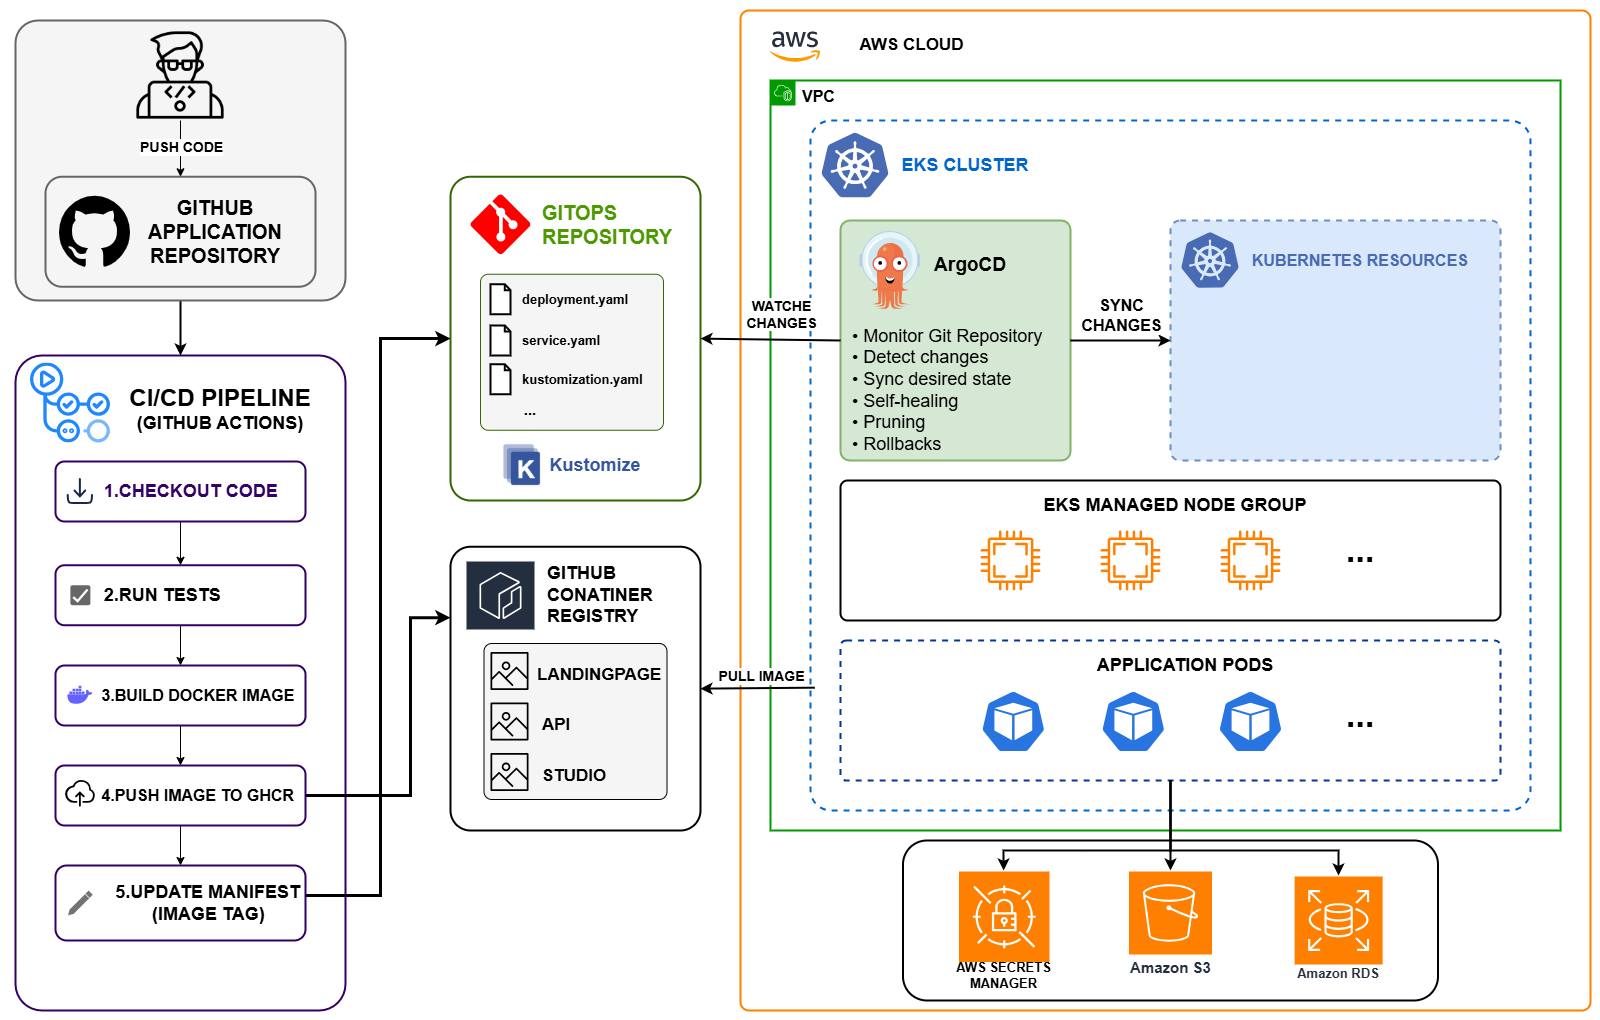
\includegraphics[width=1\linewidth]{src/assets/diagrams/arch.png}
    \caption{DevOps-Integrated Cloud Architecture.}
    \label{fig:Architecture-Overview}
\end{figure}

The system can be understood through four main workflows:

\begin{itemize}
    \item \textbf{Continuous Integration:} When a developer pushes code to 
GitHub, a GitHub Actions pipeline automatically runs tests, builds a Docker 
image, pushes it to the GitHub Container Registry, and updates the deployment 
manifest with the new image tag.

    \item \textbf{GitOps Delivery:} The GitOps repository holds all Kubernetes 
manifests and acts as the source of truth for the cluster state. ArgoCD 
watches this repository and automatically syncs any changes to the cluster. 
It also handles rollbacks and self-healing if something goes wrong.

    \item \textbf{Cluster Workloads:} Applications run as separate pods inside 
the EKS cluster on an AWS-managed node group. Each pod, whether the landing 
page, the API, or the studio, is deployed and scaled independently.

    \item \textbf{Data and Secret Management:} Persistent data is stored in 
Amazon RDS, credentials are managed through AWS Secrets Manager and injected 
directly into the relevant pods, and media files are stored in Amazon S3 and 
accessed via presigned URLs to reduce load on the cluster.
\end{itemize}

Together, these workflows cover the full lifecycle of a change, from a 
developer pushing code to the update being live in the cluster, 
while keeping the system secure, scalable, and easy to operate.

\subsection{Container Orchestration and Migration}

The legacy infrastructure ran all components of The Mashroom platform on a 
single virtual machine. This meant that any failure or update to one component 
would affect the entire system, and there was no way to scale individual parts 
independently. For this reason, we first proceeded with container orchestration and migration.

\begin{quote}

\textbf{Containerization with Docker:}
The first step was to package each application into a Docker image. A Docker 
image bundles the application with everything it needs to run, making it 
portable and consistent across any environment. This eliminates the classic 
problem of code that works on one machine but fails on another.

\textbf{Orchestration with Kubernetes:}
Once the applications were containerized, Kubernetes was used to manage and 
run them on a cluster. Each application is defined as a Deployment, which 
controls how many instances are running at any time. Services expose these 
applications internally within the cluster, while an Ingress manages external 
traffic and routes requests to the right application. Kubernetes also handles 
auto-scaling, automatically adjusting the number of running instances based 
on traffic load.

\textbf{Managed Kubernetes on Amazon EKS:}
Rather than setting up and maintaining a Kubernetes cluster manually, Amazon 
Elastic Kubernetes Service (EKS) was used. EKS is a managed service, meaning 
AWS handles the control plane, which is the part of Kubernetes responsible for 
making decisions about the cluster. This reduces operational overhead and 
ensures high availability and scalability out of the box.

\end{quote}
\subsection{Reproducible Cloud Infrastructure}
One of the key requirements identified in Section \ref{sec:Proposed solution} was the 
ability to recreate the entire infrastructure automatically, without any manual 
intervention. This is achieved using Terraform, which allows every AWS resource 
to be defined as code and provisioned automatically from scratch at any time.

The AWS infrastructure is fully described in versioned Terraform files, covering 
all the components the platform depends on: the EKS cluster, the network layer 
(VPC and subnets), AWS Secrets Manager, 
RDS, and S3. To keep the codebase structured and maintainable, the code is 
organized into modules, each responsible for a distinct part of the 
infrastructure, as illustrated in Figure \ref{fig:terraform-modules}.

\begin{figure}[H]
    \centering
    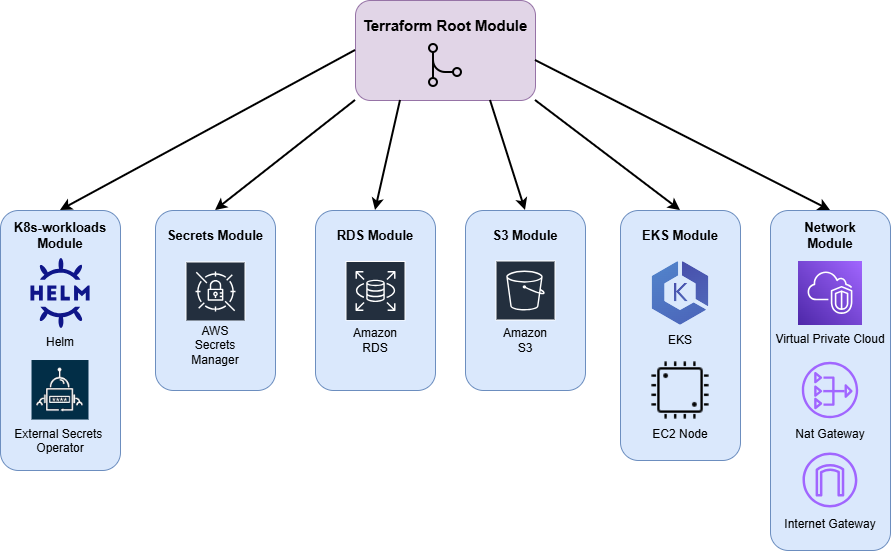
\includegraphics[width=0.75\linewidth]{src/assets/images/terraform.png}
    \caption{Terraform module structure}
    \label{fig:terraform-modules}
\end{figure}

Terraform also maintains a state file that tracks the current state of the
infrastructure, which is stored in an S3 bucket to ensure it remains shared
and consistent across the team. Finally, sensitive application credentials are
managed through the External Secrets Operator, which automatically pulls secret
values from AWS Secrets Manager and injects them into the cluster, eliminating
the need for manual secret synchronization and saving valuable development time.

\subsection{Automated and Reversible Delivery}
\label{subsec:automated_delivery}
The delivery layer is built around two complementary processes: 
Continuous Integration (CI) and Continuous Deployment (CD). 
The CI pipeline automates the building, testing, and publishing 
of application images, while the CD process ensures the cluster 
is always aligned with the latest desired state defined in the 
GitOps repository. Together they form a fully automated delivery 
pipeline where a code change is the only manual step required. 
Any bad release can also be reverted by simply reverting a commit 
in the repository, with no manual intervention on the cluster.

\subsubsection{Continuous Integration Pipeline}
Each of the three applications of The Mashroom has a dedicated CI pipeline 
powered by GitHub Actions. When new code is pushed, GitHub spins up 
a runner, which is a virtual machine that executes the pipeline steps 
automatically.

The pipeline starts by running linting and tests to verify code 
quality, then builds a Docker container image and pushes it to the 
GitHub Container Registry (GHCR). Figure~\ref{fig:ci-pipeline} 
provides an overview of this process.

\begin{figure}[H]
    \centering
    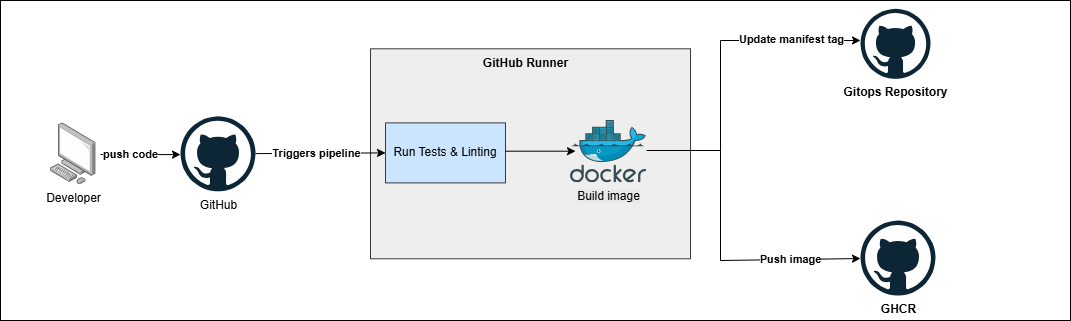
\includegraphics[width=\linewidth]{src/assets/images/ci.png}
    \caption{Continuous Integration pipeline overview}
    \label{fig:ci-pipeline}
\end{figure}

The tagging strategy differs slightly per application. The backend 
API is tagged with \texttt{dev} for staging and \texttt{main} for 
production. The frontend applications, Studio and Landing Page, are tagged only with 
\texttt{main}, as they are deployed to production only.

Once the image is pushed, the pipeline automatically updates the 
image tags in the GitOps repository, which triggers the deployment 
process described in the next section.

\subsubsection{GitOps Deployment Workflow}
Once the CI pipeline finishes, the CD process takes over. Argo CD 
\cite{argocd} runs inside the EKS cluster and continuously watches 
the GitOps repository. It compares the repository contents with the 
current state of the cluster and automatically syncs any difference 
it detects, making the repository the single source of truth for 
everything running in the cluster.

The GitOps repository holds the full cluster configuration for all 
three applications. Environment differences between staging and 
production are managed through Kustomize \cite{kustomize} overlays, 
which keep a shared base and let each environment override only what 
is strictly necessary, such as image tags, namespaces, and ingress 
hostnames. The same overlays are also used locally to validate the 
configuration before it reaches the cloud. Figure~\ref{fig:cd_workflow} 
illustrates this workflow.

\begin{figure}[H]
    \centering
    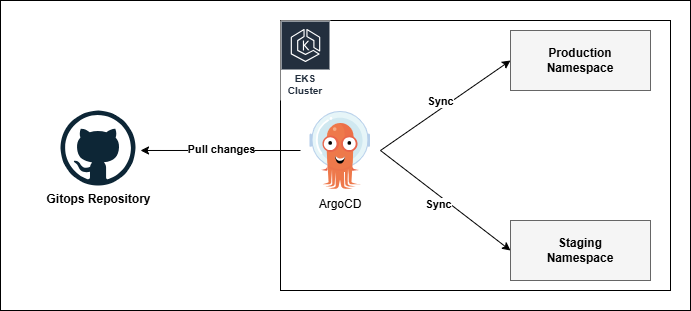
\includegraphics[width=\linewidth]{src/assets/images/cd.png}
    \caption{GitOps Deployment with Argo CD}
    \label{fig:cd_workflow}
\end{figure}

\subsubsection{Automated Rollbacks}
Because the cluster state is entirely driven by the GitOps repository, 
rolling back a bad release requires no manual action on the cluster. 
Argo CD continuously monitors the repository and syncs the cluster 
to match it. If a faulty image tag is merged, reverting that commit 
in the repository is enough to restore the previous state. Argo CD 
detects the change and automatically re-syncs the cluster to the 
last known good version.
% ----------------------------------- SECTIONS (^) ----------------------------------- %

\setcounter{secnumdepth}{0} % Set the section counter to 0 so next section is not counted in toc
% ----------------------- Conclusion ----------------------- %
\section{Conclusion}
This chapter presented the architectural decisions made for the project. 
After comparing the available tools in each domain, a stack was selected 
based on the specific requirements of the project: Terraform for infrastructure 
provisioning, Docker and Kubernetes on AWS EKS for containerization and 
orchestration, GitHub Actions for continuous integration, and ArgoCD with 
Kustomize for GitOps-based delivery. The following chapter covers the practical 
implementation of this architecture.
%In this chapter, we established the theoretical and technical foundations for our project by examining DevOps practices, containerization, infrastructure as code, CI/CD pipelines, and GitOps principles. We then conducted a comparative analysis of the tools available in each domain: Git for version control, Docker for containerization, Kubernetes for orchestration, Kustomize for configuration management, GitHub Actions for CI/CD, Terraform for infrastructure provisioning, and AWS as the cloud platform.

%Each choice was justified against the specific requirements of our project: migrating a monolithic application to a scalable, cloud-native architecture while optimizing for cost, maintainability, and automation. These tools and practices form the technical stack that will be implemented in the subsequent chapters.